\section{Ricerca di fisica Behind Standard Model con i VAEs}
\label{fisica_BSM_VAEs}

In quest'ultimo capitolo verrà presentata una possibile applicazione dei Variational Autoencoders nel campo della fisica delle alte energie, con lo scopo di ricercare segnali di nuova fisica BSM, ovvero oltre il Modello Standard. \\
Come noto, gli esperimenti portati avanti al \textit{Large Hadron Collider} hanno l'obiettivo di esplorare la fisica spingendosi sempre a più alte energie; attualmente, dopo la scoperta del \textit{Bosone di Higgs}, la teoria del Modello Standard sembrerebbe essere completa, anche se rimango alcuni problemi aperti, come lo \textit{Hierarchy Problem} e la spiegazione dell'origine della \textit{Dark Matter}. \\
Nella ricerca di nuova fisica possono essere portati avanti due approcci, detti \textit{model dependent} e \textit{model independent}. Nel primo caso la ricerca di nuova fisica avviene con un particolare modello in mente ed i risultati sono ottimi nel caso in cui il modello utilizzato è corretto, come per la scoperta del Bosone di Higgs; il limite di una ricerca di questo tipo è chiaramente dovuto al fatto che i risultati sono strettamente legati alla bontà della teoria stessa. Dall'altro lato una ricerca model independent ha il pregio di non essere legata ad una particolare teoria fisica e quindi è capace di ricercare eventuali segnali di nuova fisica a prescindere da un modello teorizzato in anticipo.\\
Nelle pagine seguenti si cercherà di capire se è possibile addestrare un Variational Autoencoder sugli eventi di background (ovvero sulla fisica prevista dal Modello Standard) in modo che sia capace di rilevare eventuali segnali di nuova fisica come delle anomalie. L'approccio seguito è da un lato model dependent, nel senso che i dati utilizzati sono prodotti attraverso simulazioni Montecarlo in base alla SUSY (\textit{Supersimmetry theory}) per la ricerca della coppia di particelle fermione/bosone (chargino e gluino), e dall'altro model independent, perché le masse di queste due particelle non sono stabilite e quindi la ricerca deve essere sensibile a tutte le varie combinazioni possibili.
Successivamente, nel caso in cui l'algoritmo si dimostri efficace nella discriminazione del segnale usando le simulazioni MC, è ragionevole pensare di estendere l'applicazione di questo metodo direttamente sui dati sperimentali prodotti al Large Hadron Collider. Questo ulteriore passaggio è possibile solo in virtù dell'approccio \textit{Unsupervised} per cui non è necessario dare all'algoritmo le etichette fondo/segnale durante la fase di training. Sarebbe infatti impensabile avere in anticipo questa informazione per i dati sperimentali. Per lo stesso motivo si capisce perché un algoritmo \textit{Supervised} non possa essere in generale direttamente applicato ai dati sperimentali; infatti, questa seconda categoria di modelli richiede nella fase di training le etichette fondo/segnale per ciascun evento fisico al fine di impararne la distinzione. Si deve perciò ricorrere necessariamente alle simulazioni MC con tutte le incertezze modellistiche annesse.
\newpage

\subsection{Dataset}
\label{dataset}
Per l'addestramento del modello e per la successiva fase di verifica sono stati utilizzati i dati prodotti attraverso simulazioni Montecarlo (MC), in base alla teoria di riferimento (SUSY). Le variabili fisiche che definiscono ogni evento sono otto ($\textit{met}$, $\textit{mt}$, $\textit{mbb}$, $\textit{mct2}$, $\textit{mlb1}$, $\textit{lep1Pt}$, $\textit{njet30}$, $\textit{nBjet30-MV2c10}$) e sono le stesse utilizzate nell'analisi fisica relativa allo studio \cite{susy_alberto}. Di conseguenza lo spazio iniziale, che dovrà essere compresso dal VAE, sarà 8-dimensionale. \\
Attraverso la simulazione MC vengono prodotti eventi sia di background che di segnale e, nel caso in cui l'algoritmo sia capace di discriminare tra eventi di fondo e di segnale, potrà essere applicato ai dataset reali, nei quali chiaramente non vi è questo tipo di differenziazione.\\ 
Prima di passare alla fase di codifica, gli eventi (sia di segnale che di background) sono stati sottoposti ad una serie di tagli di preselezione sulle variabili, come riportato nella tabella~\ref{tab:tagli di preselezione}.

\begin{table}[h!]
	\centering
	\begin{tabular}{lc}
		\hline
		&Preselezione \\
		\hline
		Esattamente un leptone di segnale&Vero\\
		met\ trigger&Vero\\
		$2-3$ jets con $p_{T}>30 GeV$&Vero\\
		$b$-tagged jet&[1-3]\\
		met\ &$> 220$ GeV\\
		mt\ &$> 50$ GeV\\
		mbb\ &[$100-140$]GeV\\
		mct\ &$>100$GeV\\
		\hline
	\end{tabular}
	\caption{Sono riportati i tagli di preselezione applicati sia agli eventi di segnale che di background, prodotti attraverso una simulazione MC.}
	\label{tab:tagli di preselezione}
\end{table} 
Gli eventi prodotti con il metodo MC sono stati divisi, come si richiede in un processo di apprendimento automatico, in una training data set, un validation data set ed un test data set.
\newpage

\subsection{Addestramento del VAE}
\label{simulazione}
Come è stato detto nelle sezioni precedenti, il VAE deve essere addestrato in modo tale da rilevare eventuali indizi di fisica BSM come delle anomalie, cercando di dimostrarsi sensibile ad una ampia gamma di possibili segnali. Ma perché un tale compito non può essere svolto da un algoritmo di apprendimento supervisionato?\\
Un classificatore binario, ovvero un modello capace di discriminare fra due sole categorie (segnale e background), viene addestrato su un training data set i cui eventi di segnale sono generati facendo riferimento ad un determinato modello; in questo modo il classificatore è in grado di discriminare solo gli eventi di segnale compatibili con quel particolare modello, tuttavia quando ne verranno presentati altri prodotti con diversi modelli, allora la classificazione risulterà totalmente arbitraria ed è qui che si evince il limite principale di una ricerca model dependent. Un ulteriore vantaggio del VAE ed in generale degli approcci model dependent, rispetto a quelli model dependent, è quello di poter essere applicato direttamente sui dati come anticipato nella sezione introduttiva di questo capito (\ref{fisica_BSM_VAEs}). In questo modo si evitano quei problemi di incertezze modellistiche legate alle simulazioni montecarlo.\\
In linea con ciò che è già stato illustrato nel capitolo~\ref{VAEs}, gli eventi di segnale e di background, che sono stati prodotti attraverso simulazioni MC, sono rappresentabili in uno spazio 8-dimensionale. Durante il processo di addestramento del VAE gli eventi di background vengono compressi nello spazio latente (tridimensionale), decompressi per essere ricostruiti e poi confrontati con quelli iniziali per il calcolo dell'errore e quindi per dare il via al processo di backpropagation (~\ref{reti neurali}). \\
Dopo la fase di addestramento si verifica che il VAE abbia imparato come ricostruire gli eventi fisici di background usati per l'addestramento, dopo averli compressi nello spazio latente. A tal proposito verranno confrontate le distribuzioni originali date in input con quelle rigenerate dalla rete. Allo stesso tempo, si ci aspetta che il modello  commetta un errore di ricostruzione maggiore quando, invece che eventi di background, vengono dati in input eventi di segnale. La limitata capacità di generalizzare su questa nuova categoria di eventi mai visti durante la procedura di addestramento dovrebbe indurre il VAE ad una ricostruzione meno accurata. Come si vedrà è possibile allora usare la distribuzione dell'errore di ricostruzione per eventi di background e segnale per discriminare tra queste due tipologie di eventi.\\
Tra i contributi originali di questa tesi vi è anche la possibilità di pesare in maniera diversa il contributo che le diverse variabili fisiche che definiscono un evento possono apportare al processo di discriminazione e, per questo motivo, verranno presentati due casi: nel primo le otto variabili avranno tutte lo stesso peso, mentre nel secondo si proverà a capire se, dando maggiore importanza ad alcune di esse, si otterrà un processo di discriminazione più efficiente. \\ 
In ogni caso, verranno illustrati i risultati ottenuti pesando tutte le variabili allo stesso modo. \\

\newpage

\subsection{Risultati}
\label{risultati}
Come primo passo bisogna capire se, a seguito del processo di addestramento, il VAE è in grado di ricostruire gli eventi di background in maniera ottimale. Il risultato del processo di ricostruzione è riportato in figura~\ref{ricostruzione}. 

\begin{figure}[h!]
	\centering
	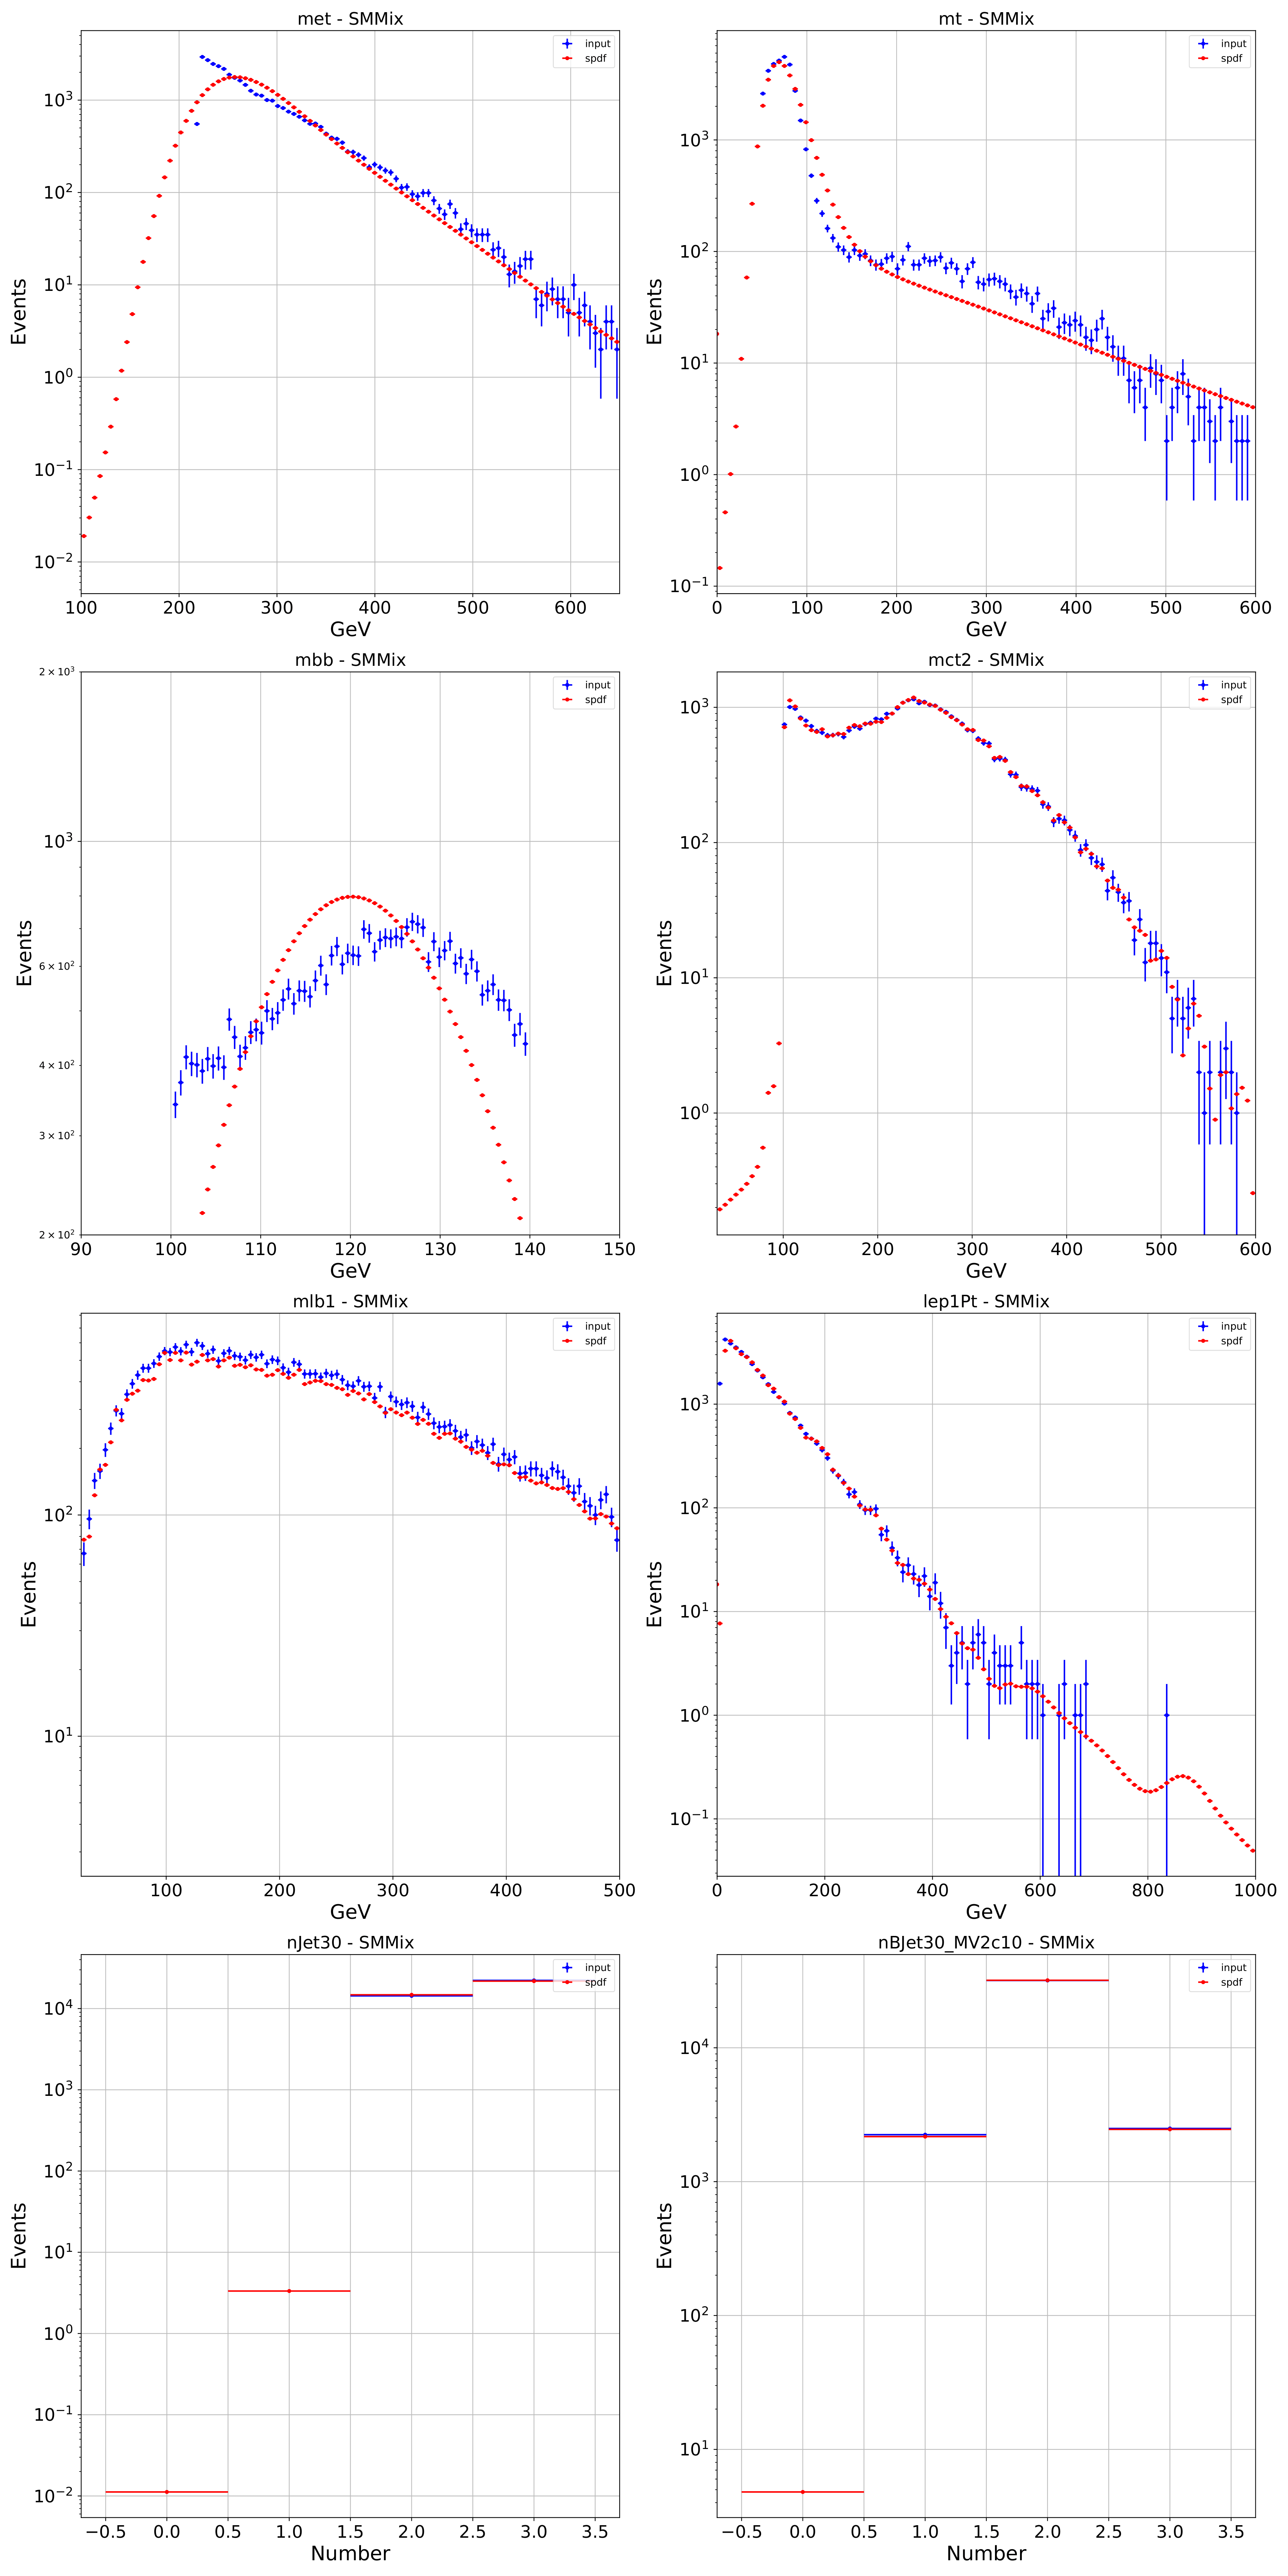
\includegraphics[width=0.64\textwidth]{figs/risultati_simulazione/ricostruzione.png}
	\caption{Confronto tra gli input in ingresso del VAE (in blu) e quelli ricostruiti (in rosso) per le otto componenti dei pattern di input.}
	\label{ricostruzione}
\end{figure}

Dall'osservazione qualitativa della figura~\ref{ricostruzione} emerge che il processo di ricostruzione del VAE risulta essere molto accurato per tutte le variabili, ad eccezione della $\textit{mbb}$. Si giunge a questa conclusione confrontando gli eventi originali (in blu) con quelli ricostruiti (in rosso). \\
Come detto, la sola variabile con ricostruzione non soddisfacente è la $\textit{mbb}$, ma questo problema può essere ovviato pesando in maniera maggiore tale variabile (per esempio impostando un peso pari a due o tre).\\
Nel complesso si può affermare che il processo di addestramento del VAE ha avuto successo e che quindi è in grado di ricostruire gli eventi di background in maniera piuttosto accurata. \\ 
Come noto, l'errore per ogni singolo evento viene calcolato sommando quello sulle otto variabili (differenza fra punto blu e rosso) e, da qui, si ottiene la distribuzione della $\textit{Loss}$. L'obiettivo è quello di ottenere una distribuzione degli errori con un picco su valori bassi della Loss. Allo stesso tempo, inserendo invece gli eventi di segnale, è auspicabile osservare una distribuzione centrata su valori della Loss maggiori (spostata quindi verso destra) al fine di ottenere una migliore selezione di questi eventi. Per verificare questa situazione si forniscono al VAE anche gli eventi di segnale (sempre generati tramite metodo MC).\\
In figura~\ref{distribuzione_loss} viene riportata la distribuzione della Loss per il segnale di background e per vari segnali di fondo relativi a diverse combinazioni delle masse del Chargino e del Gluino.

\begin{figure}[h!]
	\centering
	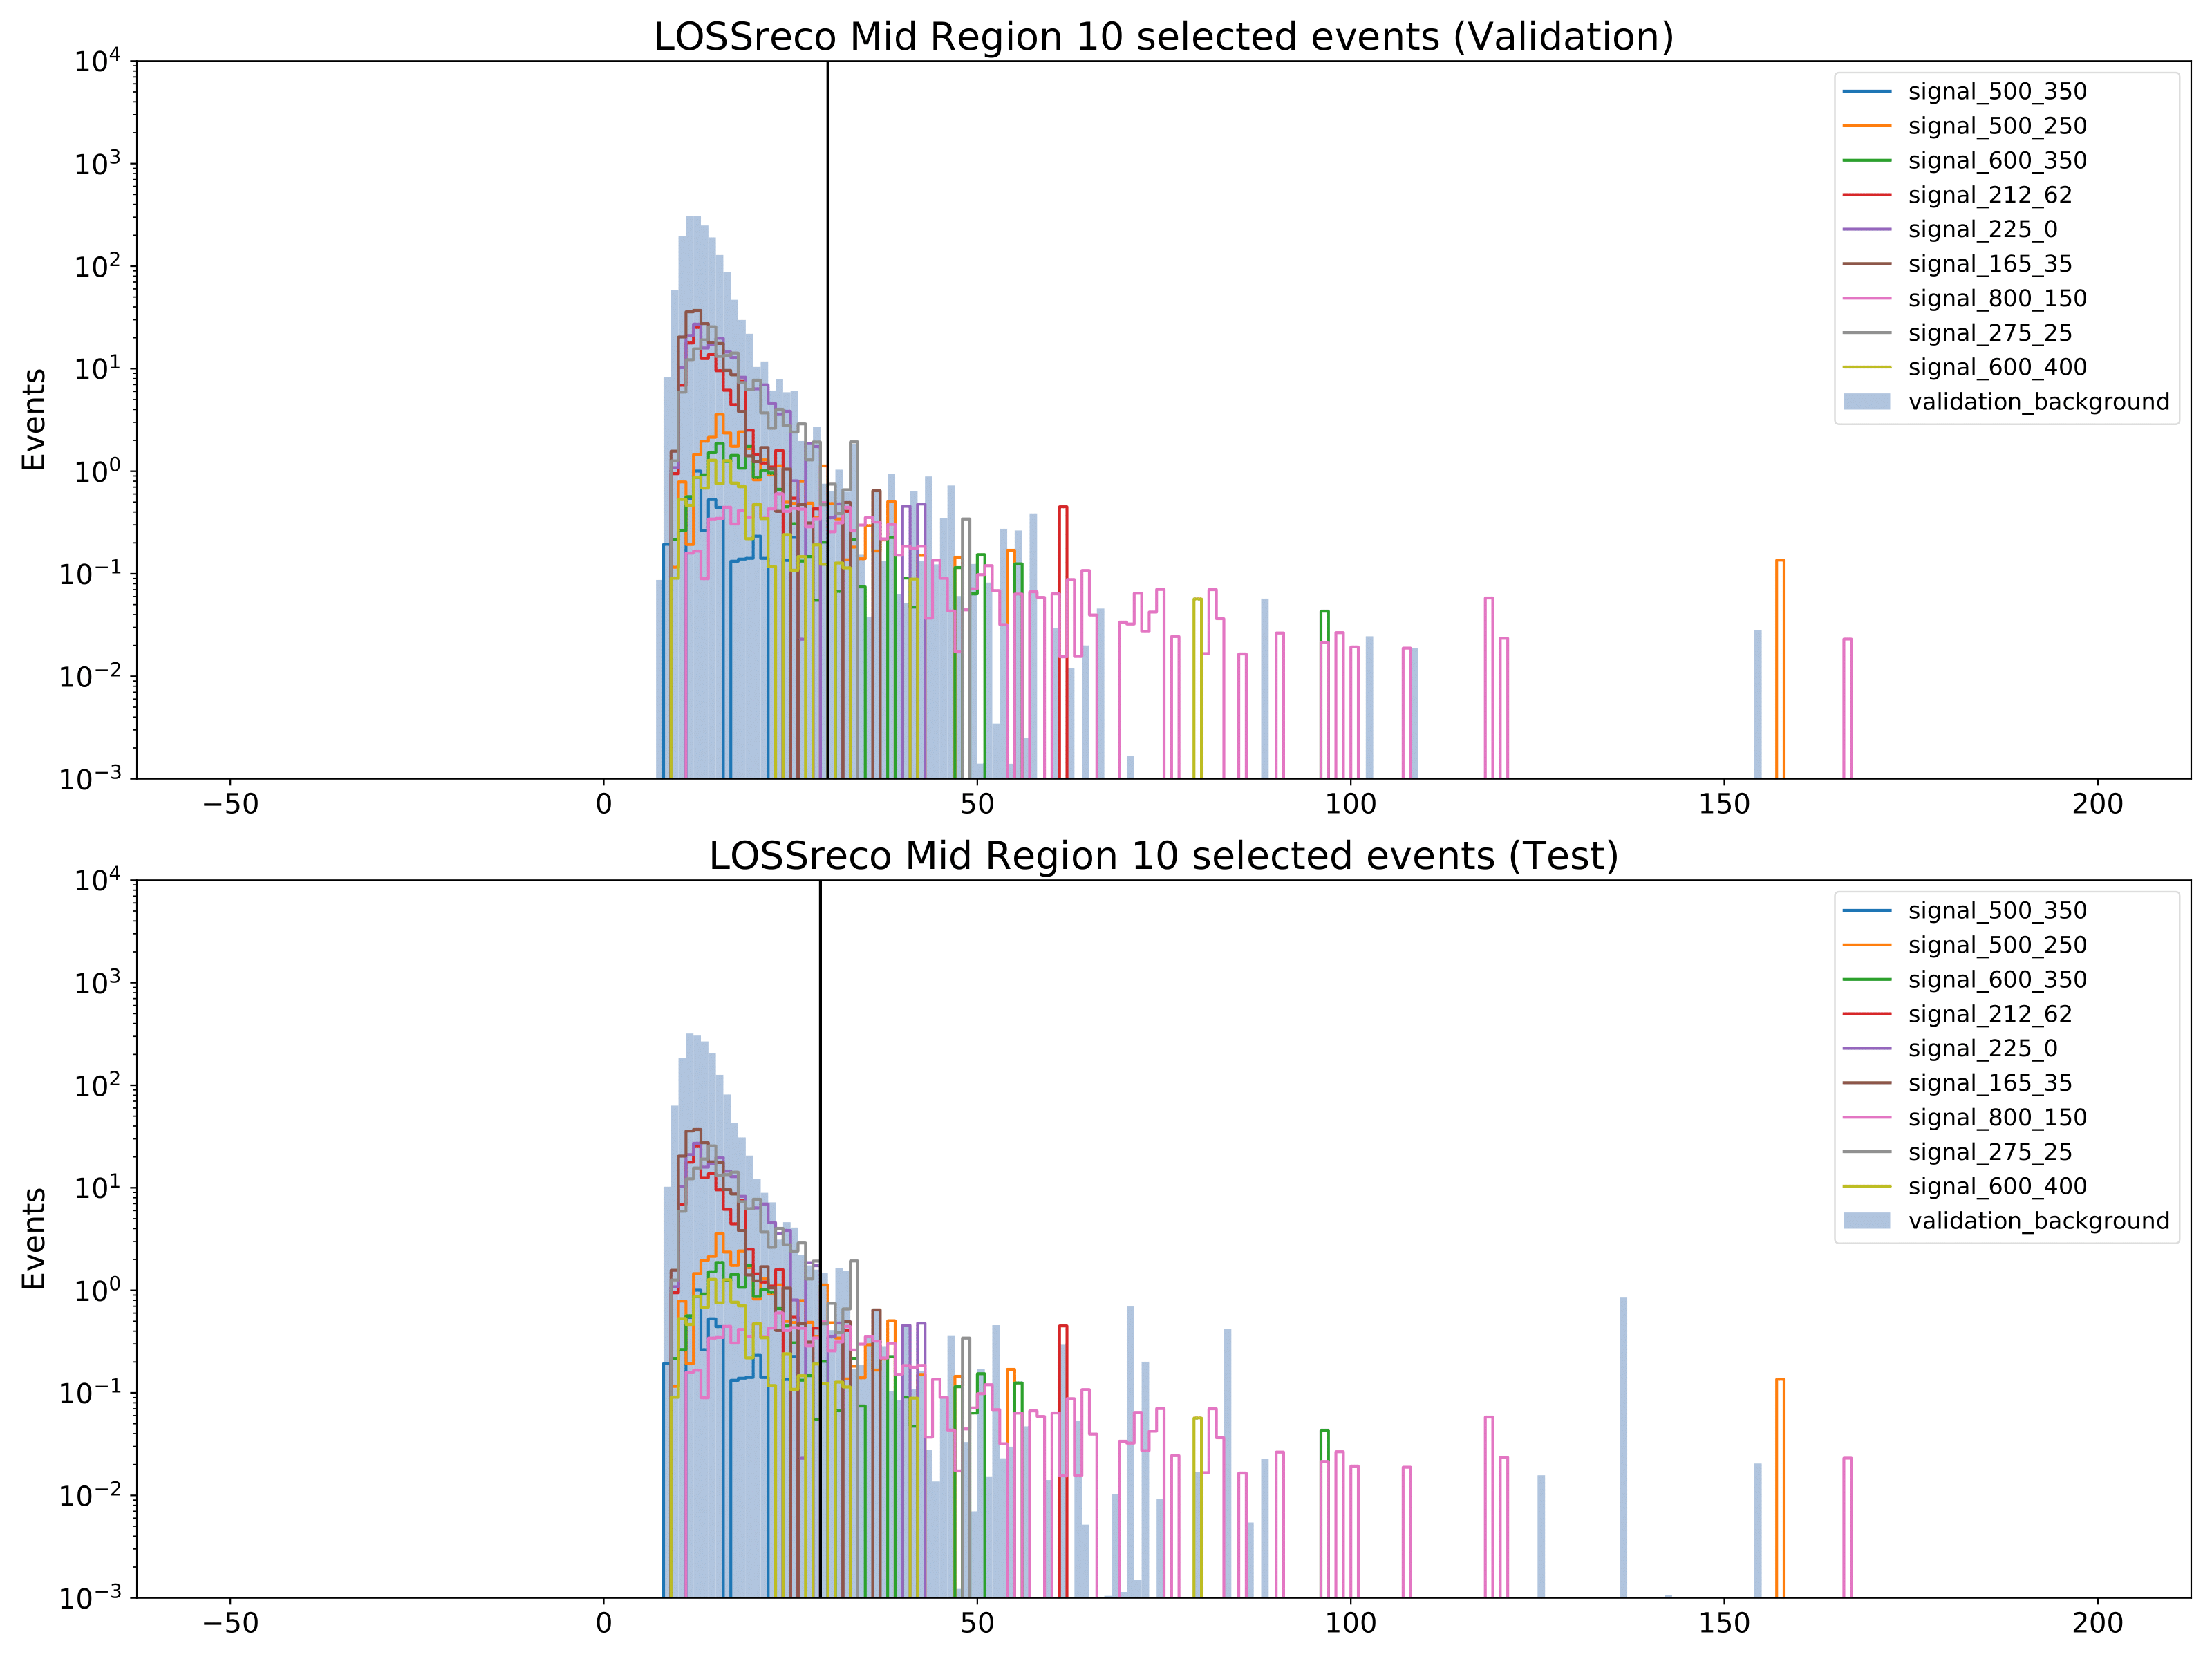
\includegraphics[width=0.99\textwidth]{figs/risultati_simulazione/distribuzioneLoss.png}
	\caption{Distribuzione della $\textit{Loss}$ per i pattern di background e per quelli di segnale relativi ad alcune combinazioni delle masse di Chargino-Gluino. La prima immagine è relativa al Vaidation data set, mentre la seconda al test data set.}
	\label{distribuzione_loss}
\end{figure}

Come prima considerazione si ottiene una conferma della qualità del processo di addestramento perché, come da attese, la distribuzione della Loss per gli eventi di background presenta un picco spostato verso sinistra, ovvero verso bassi valori dell'errore di ricostruzione. \\ 
In seconda istanza può essere fatta un'analisi qualitativa per quanto riguarda le distribuzioni della Loss per gli eventi di segnale (in figura~\ref{distribuzione_loss} sono riportate solo le distribuzioni relative ad alcune combinazioni delle masse del Chargino e del Gluino): si vede, in linea con ciò che ci si aspettava, che quasi tutte le distribuzioni degli eventi di segnale presentano dei picchi spostati verso destra rispetto a quella degli eventi di background, ma tale fenomeno non è troppo accentuato e ciò suggerisce la necessità di pesare in maniera differente le otto diverse variabili (un confronto di questo tipo verrà svolto nella prossima sezione). Bisogna notare che il fatto di trovare distribuzioni della Loss con picchi sulla sinistra per gli eventi di background e sulla destra per quelli di segnale permetterà, una volta applicato il VAE sui dati reali, per i quali la distinzione fondo-segnale non è nota a priori, di poter affermare che un evento con errore di ricostruzione alto è molto probabile che sia classificabile come segnale e non come background. \\
A questa prima analisi qualitativa ne viene fatta seguire una quantitativa, con la quale si riesce a definire per quali combinazioni delle masse delle due particelle il VAE riesce a discriminare gli eventi di segnale da quelli di background.\\
Per portare a termine questo obiettivo si imbastisce un esperimento di conteggio: viene selezionato un numero di eventi di background $N_b$ nella parte destra della distribuzione (linee nere in figura~\ref{distribuzione_loss}) e si vuole calcolare la probabilità $p(N_b + N_s|N_b)$, dopodiché se tale valore di probabilità è inferiore a 0.5 allora si afferma che è altamente improbabile che tutti gli eventi $N_b + N_s$ siano riconducibili solo al background e, di conseguenza, alcuni di questi possono essere assegnati alla categoria del segnale. \\


\color{red} (queste ultime affermazioni le devo chiedere e chiarire meglio... devo capire se è giusto questo: addestro il modello -> ottengo distribuzione della Loss per il validation ed il test -> su questa distribuzione piazzo la linea nera, ovvero seleziono un determinato numero di eventi nella parte destra -> per esempio 5 e quindi si imposta un valore x dell'errore -> di conseguenza mi aspetto mediamente 5 eventi nelle nuove misure sui dati veri -> faccio la misura e ne trovo per esempio 9 -> se la probabilità di averne 9 quando me ne aspetto 5 è <0.5 affermo che in quei 9 ci sono eventi di segnale)
\color{black} 

Le figure~\ref{test-25-50-80} e~\ref{test-100-200-400} rappresentano il risultato dell'esperimento di conteggio; lungo l'asse delle ascisse sono riportate \color{red} da chiedere \color{black} mentre lungo quello delle ordinate le \color{red} da chiedere \color{black}. Si osserva che i punti rossi rappresentano le particolari combinazioni delle masse delle due particelle per le quali il VAE è in grado di discriminare fra segnale e background, mentre in verde quelle per le quali tale discriminazione non può essere compiuta.

\newpage

\begin{figure}[h!]
	\centering
	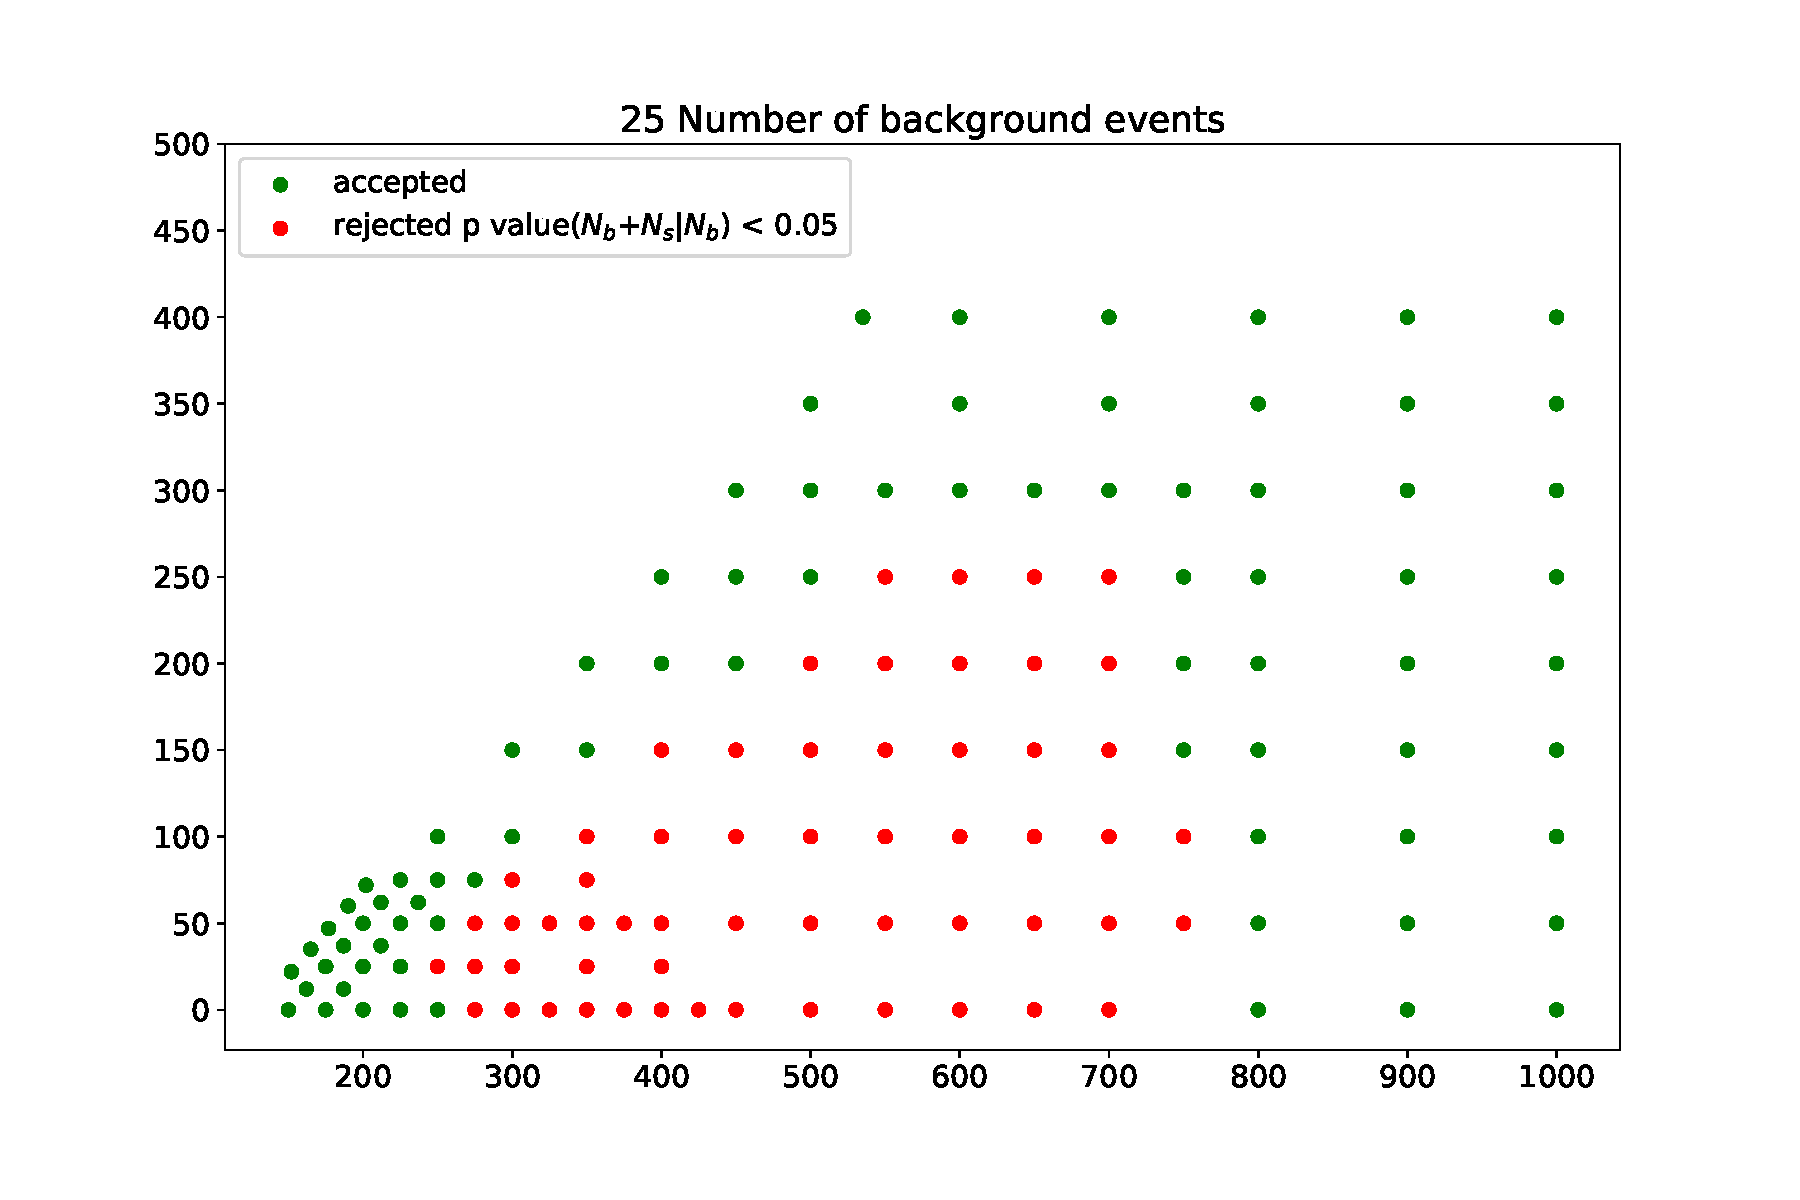
\includegraphics[width=0.72\textwidth]{figs/risultati_simulazione/25.pdf}
	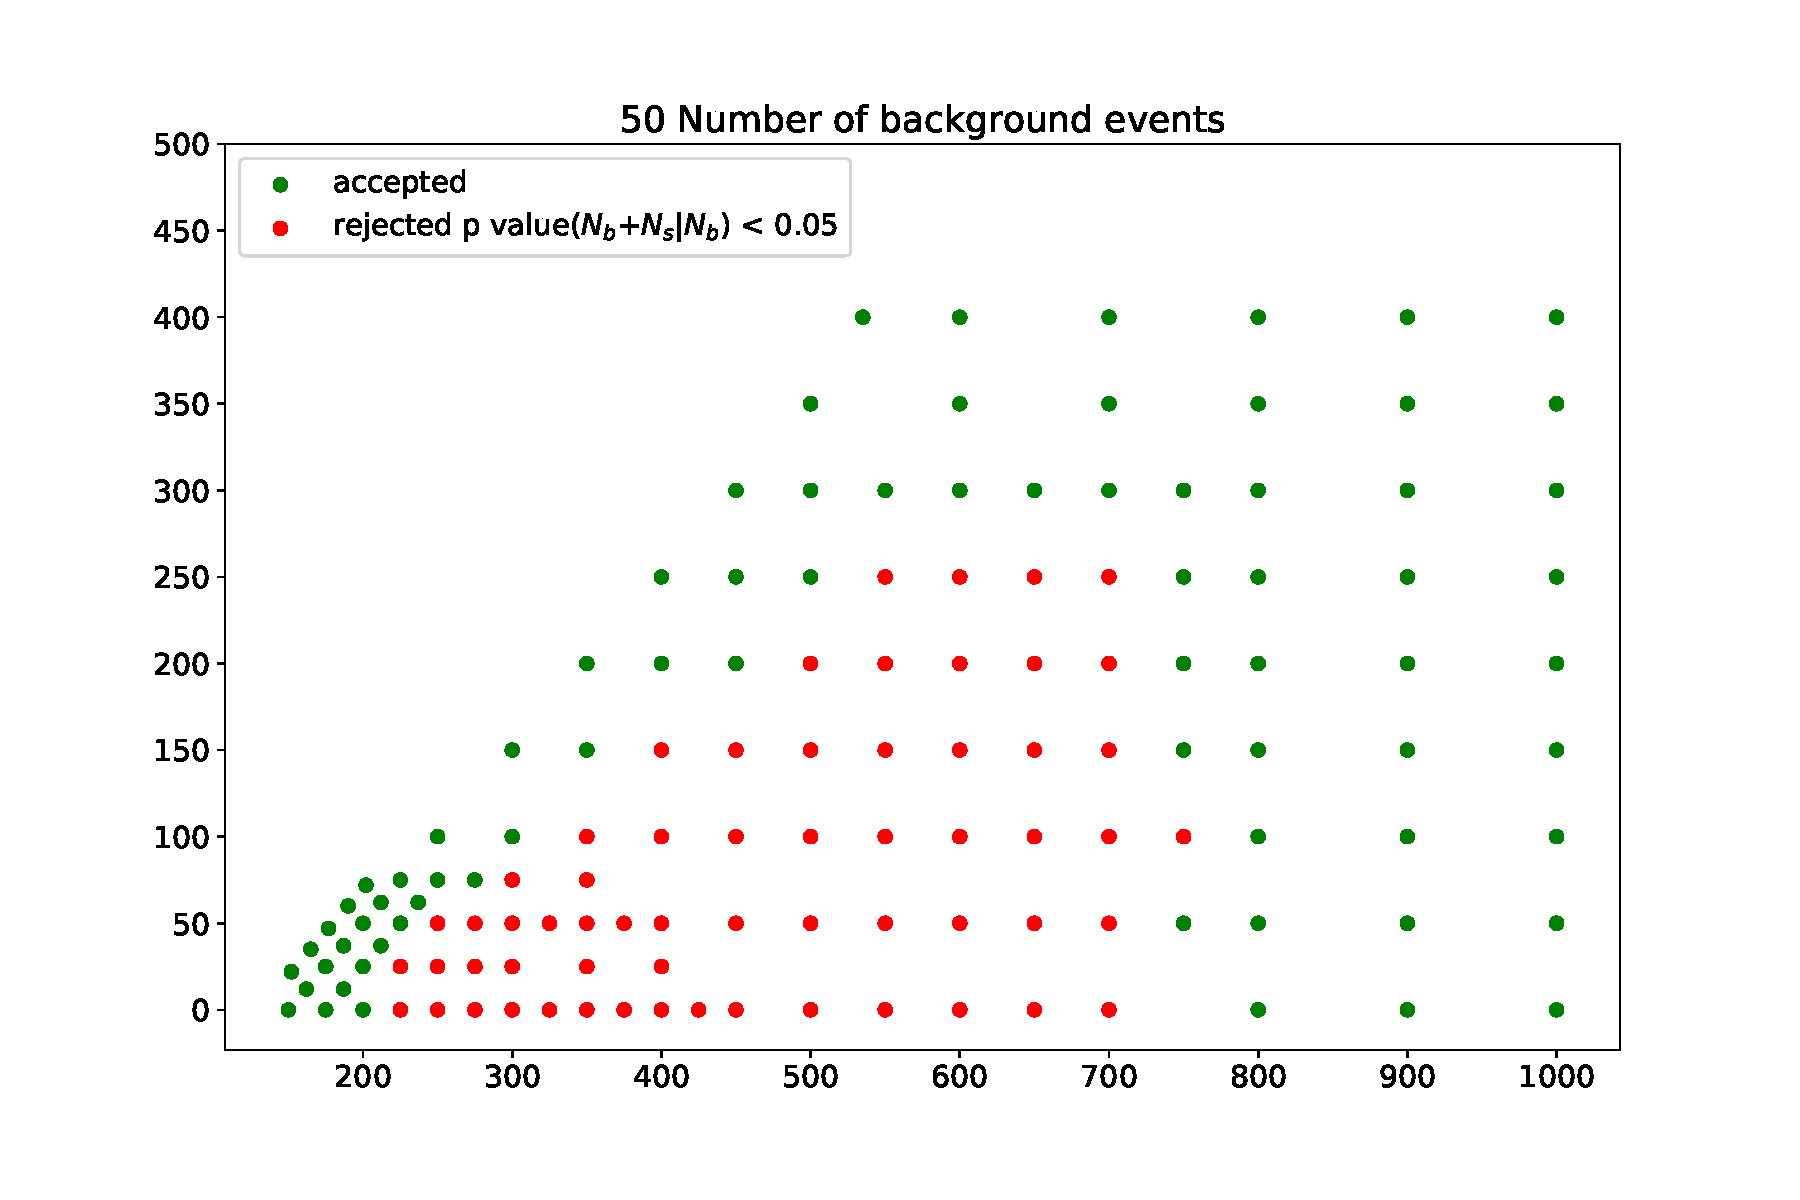
\includegraphics[width=0.72\textwidth]{figs/risultati_simulazione/50.pdf}
	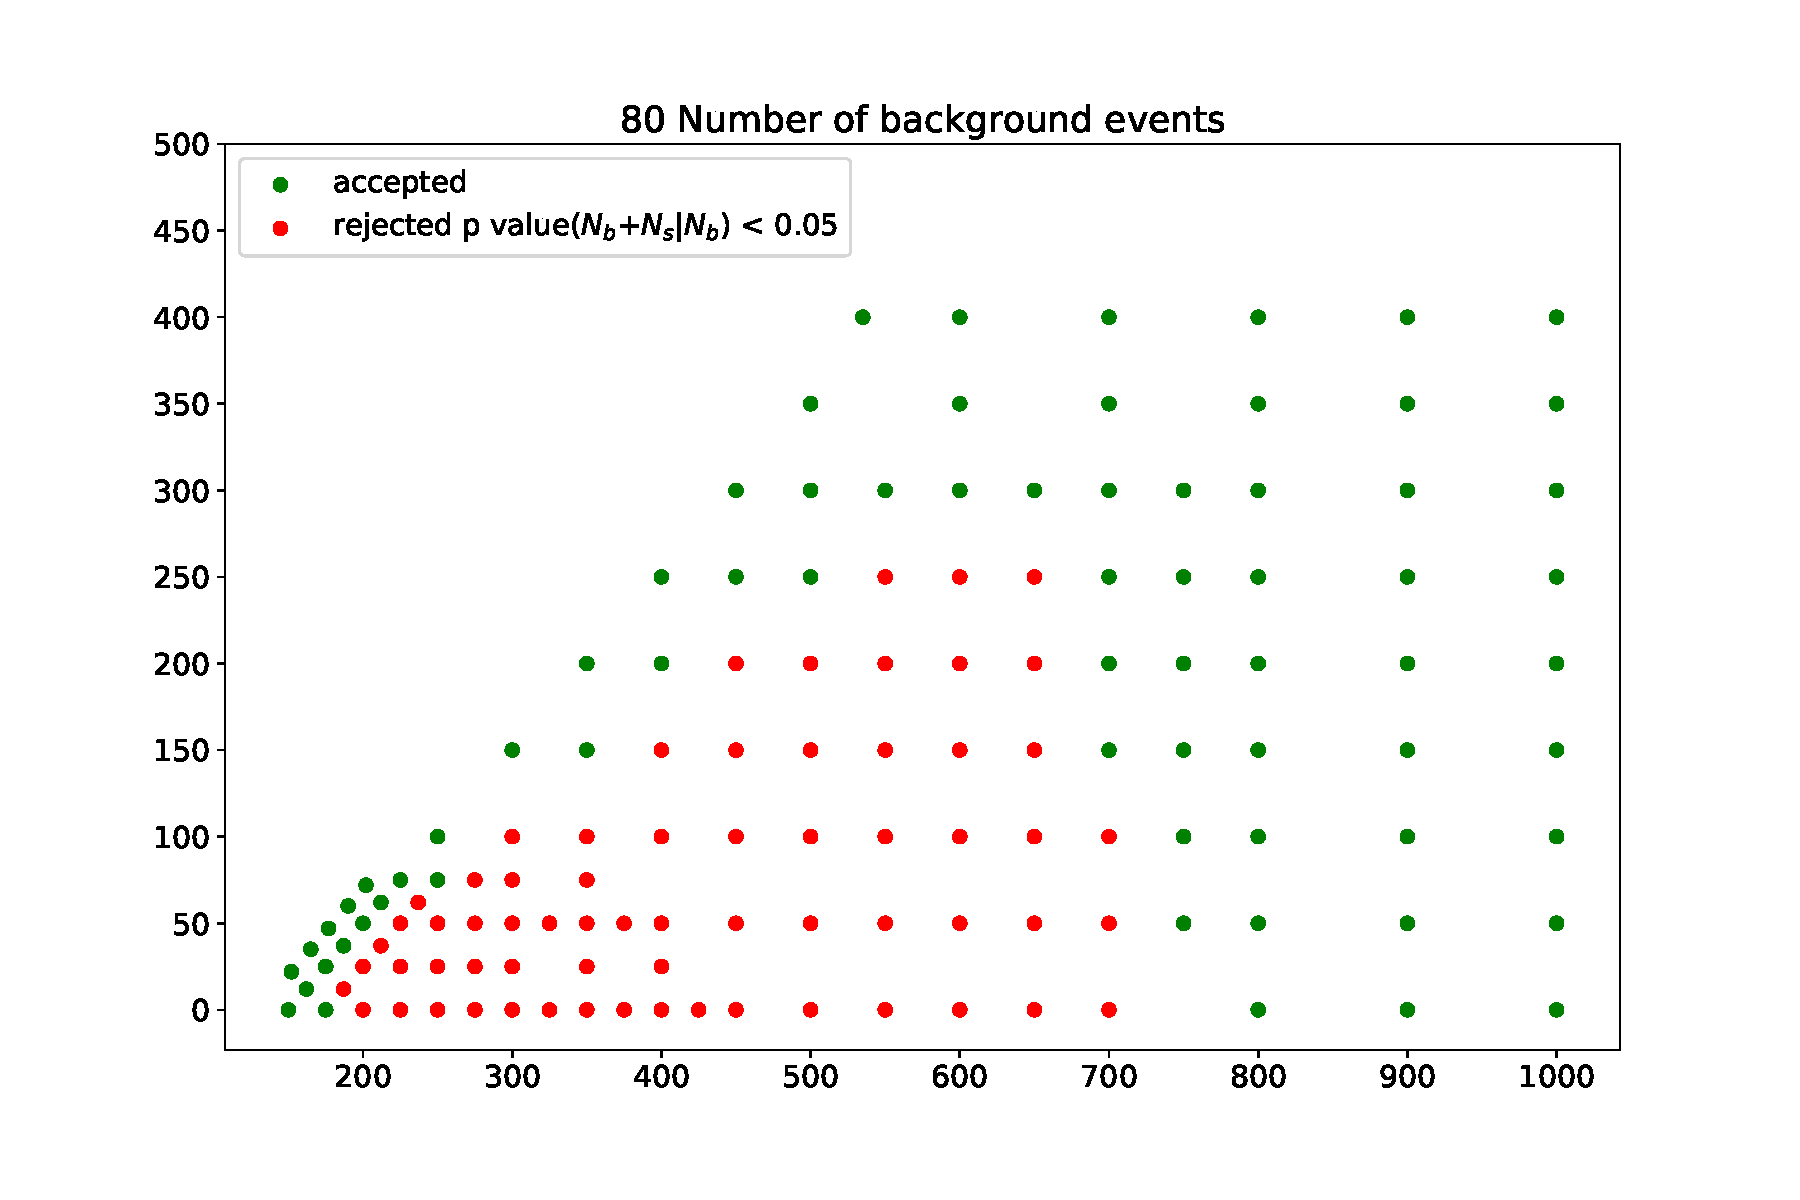
\includegraphics[width=0.72\textwidth]{figs/risultati_simulazione/80.pdf}
	\caption{Risultati degli esperimenti di conteggio per, rispettivamente, 25, 50 e 80 eventi di background selezionati nella parte destra della distribuzione della Loss.}
	\label{test-25-50-80}
\end{figure}
\begin{figure}[h!]
	\centering
	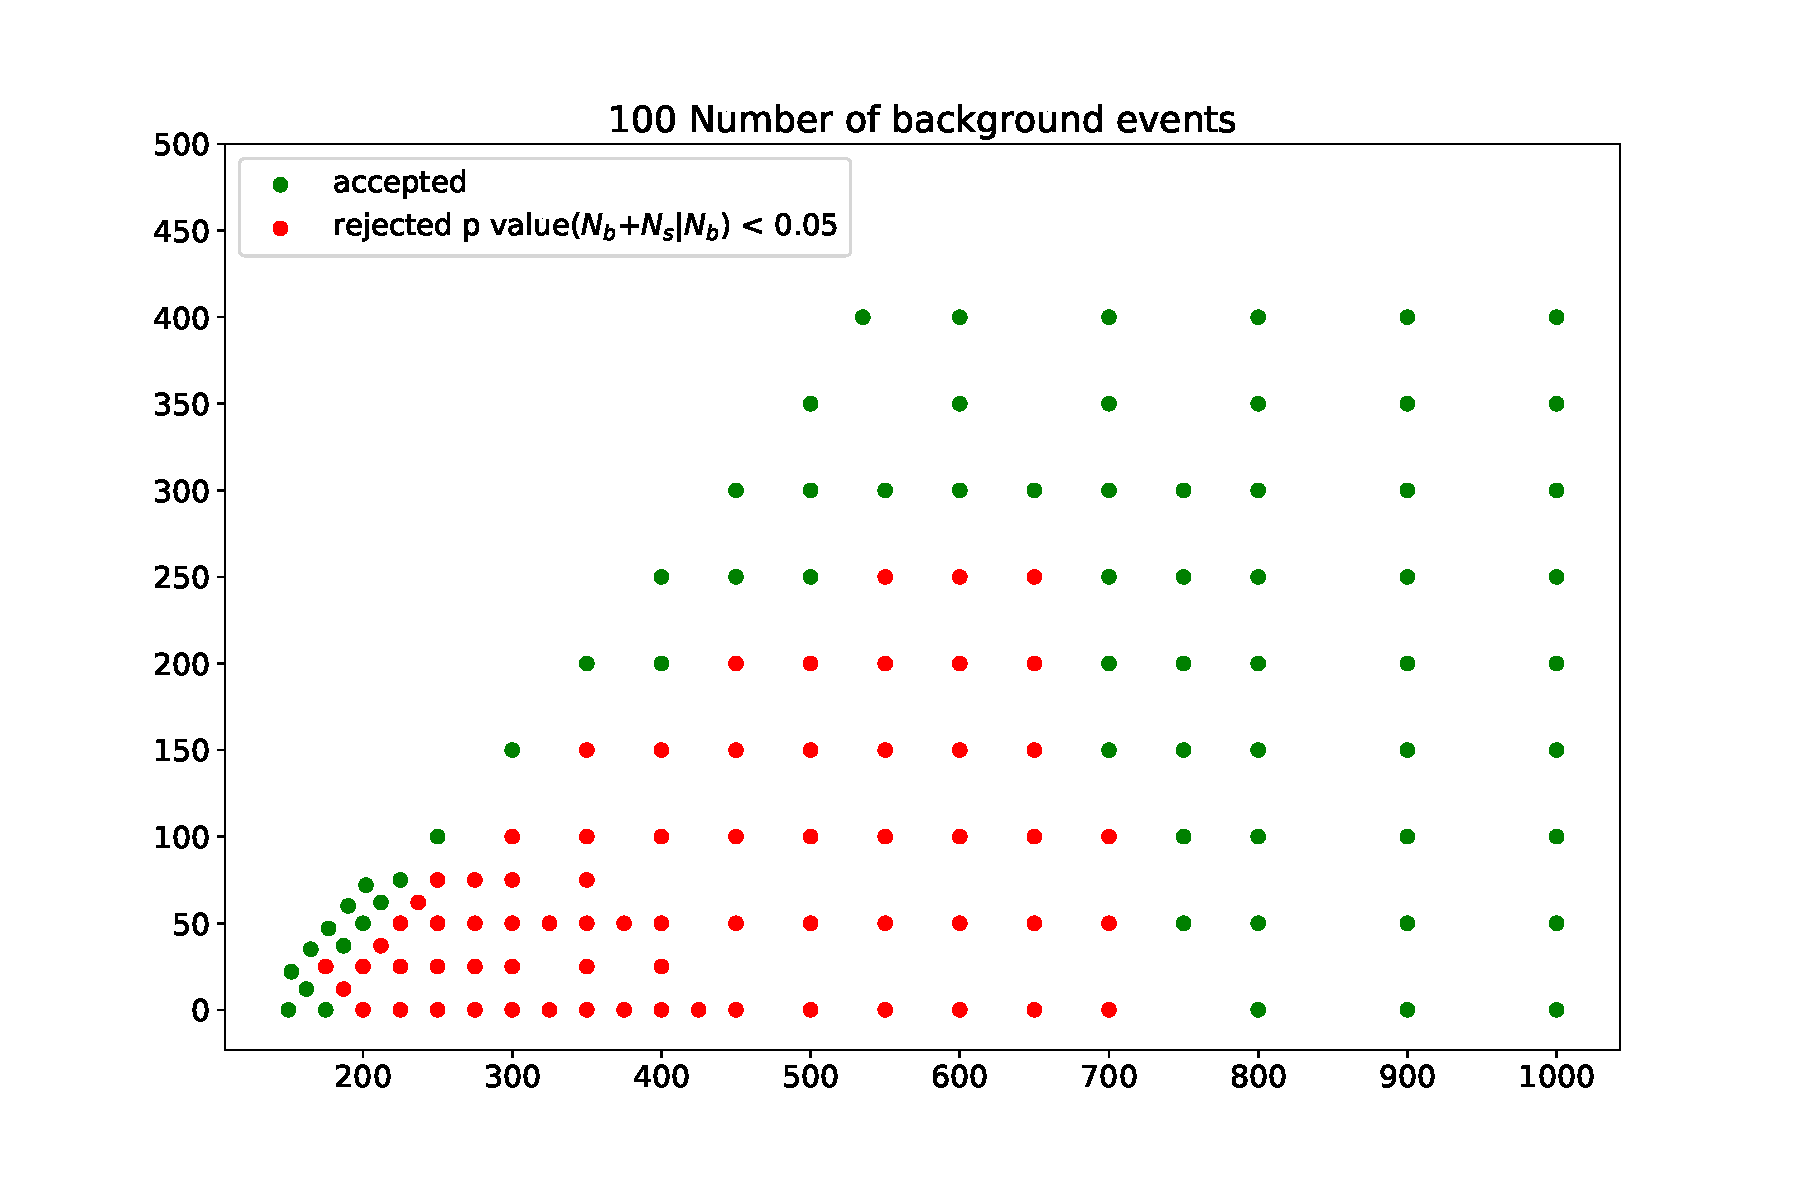
\includegraphics[width=0.71\textwidth]{figs/risultati_simulazione/100.pdf}
	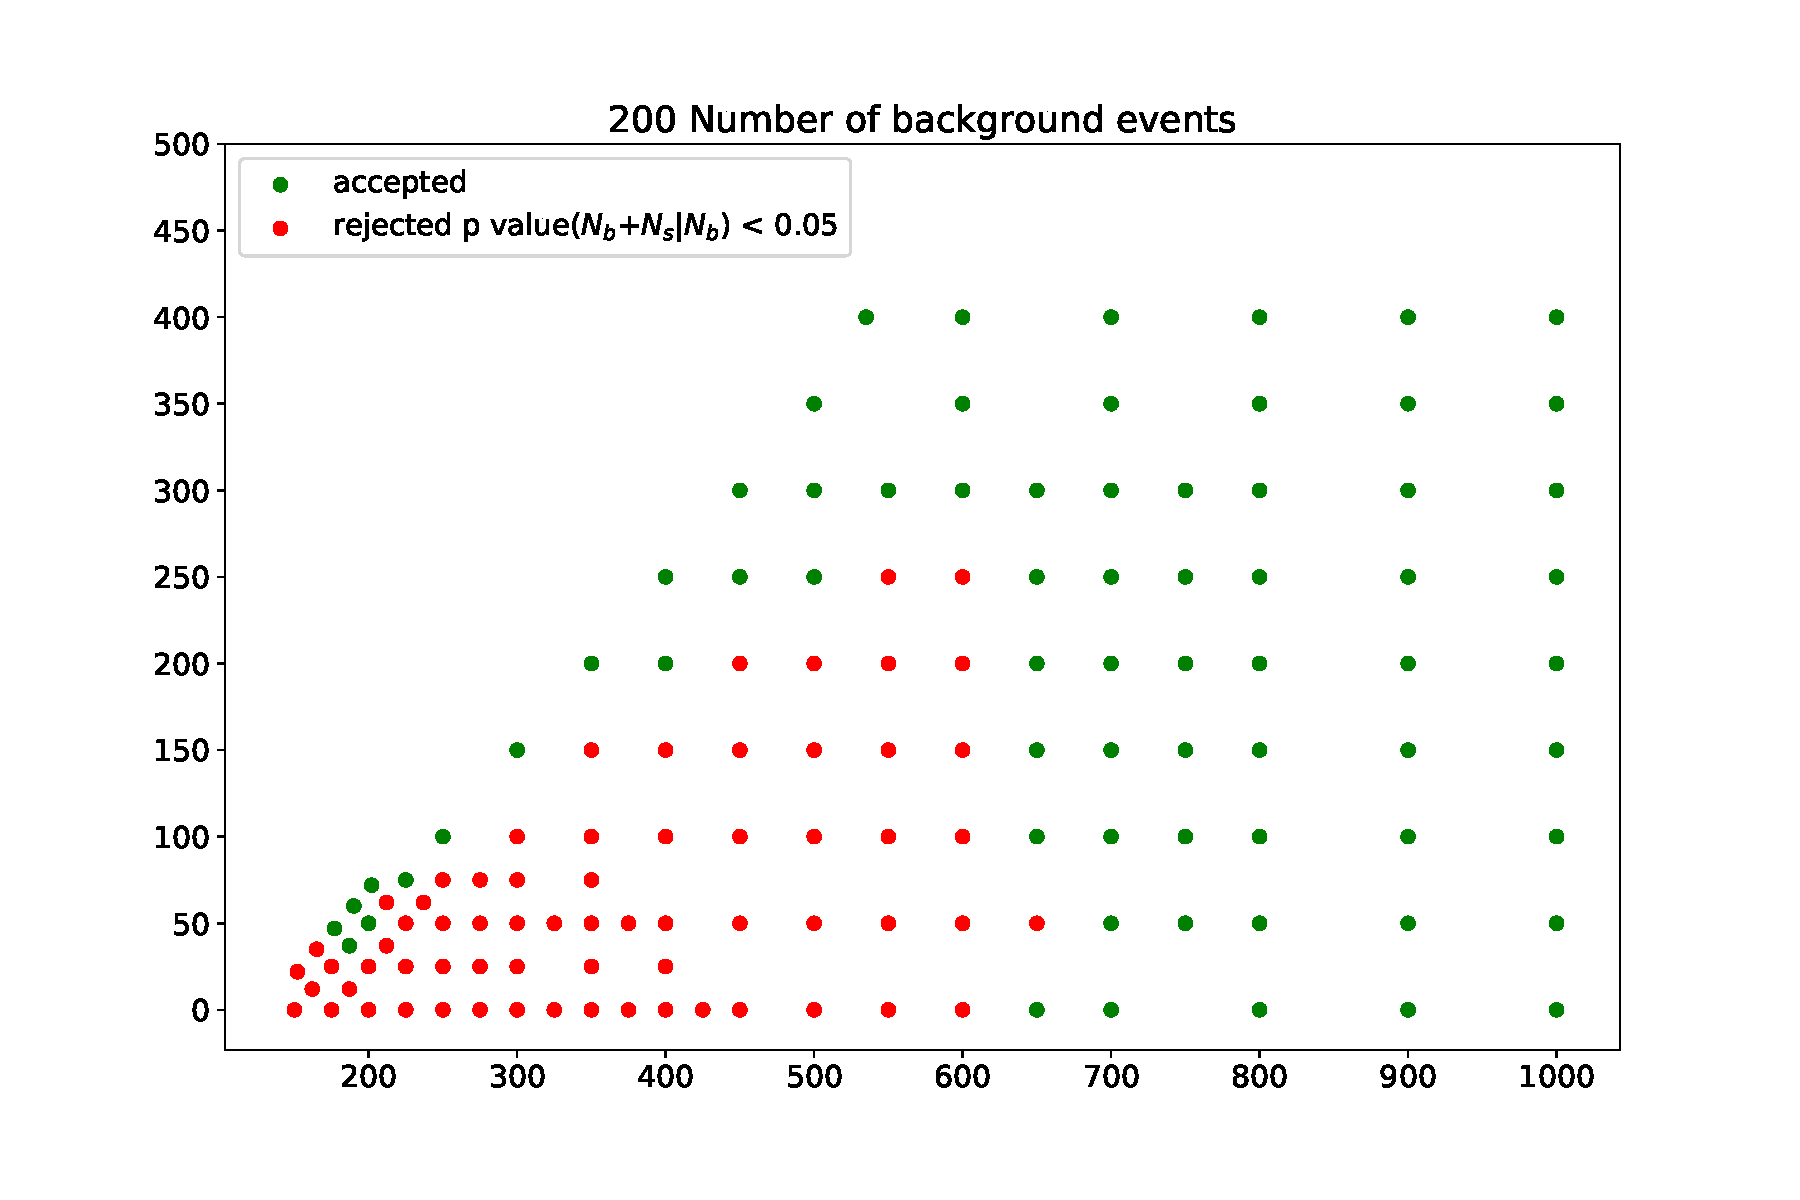
\includegraphics[width=0.71\textwidth]{figs/risultati_simulazione/200.pdf}
	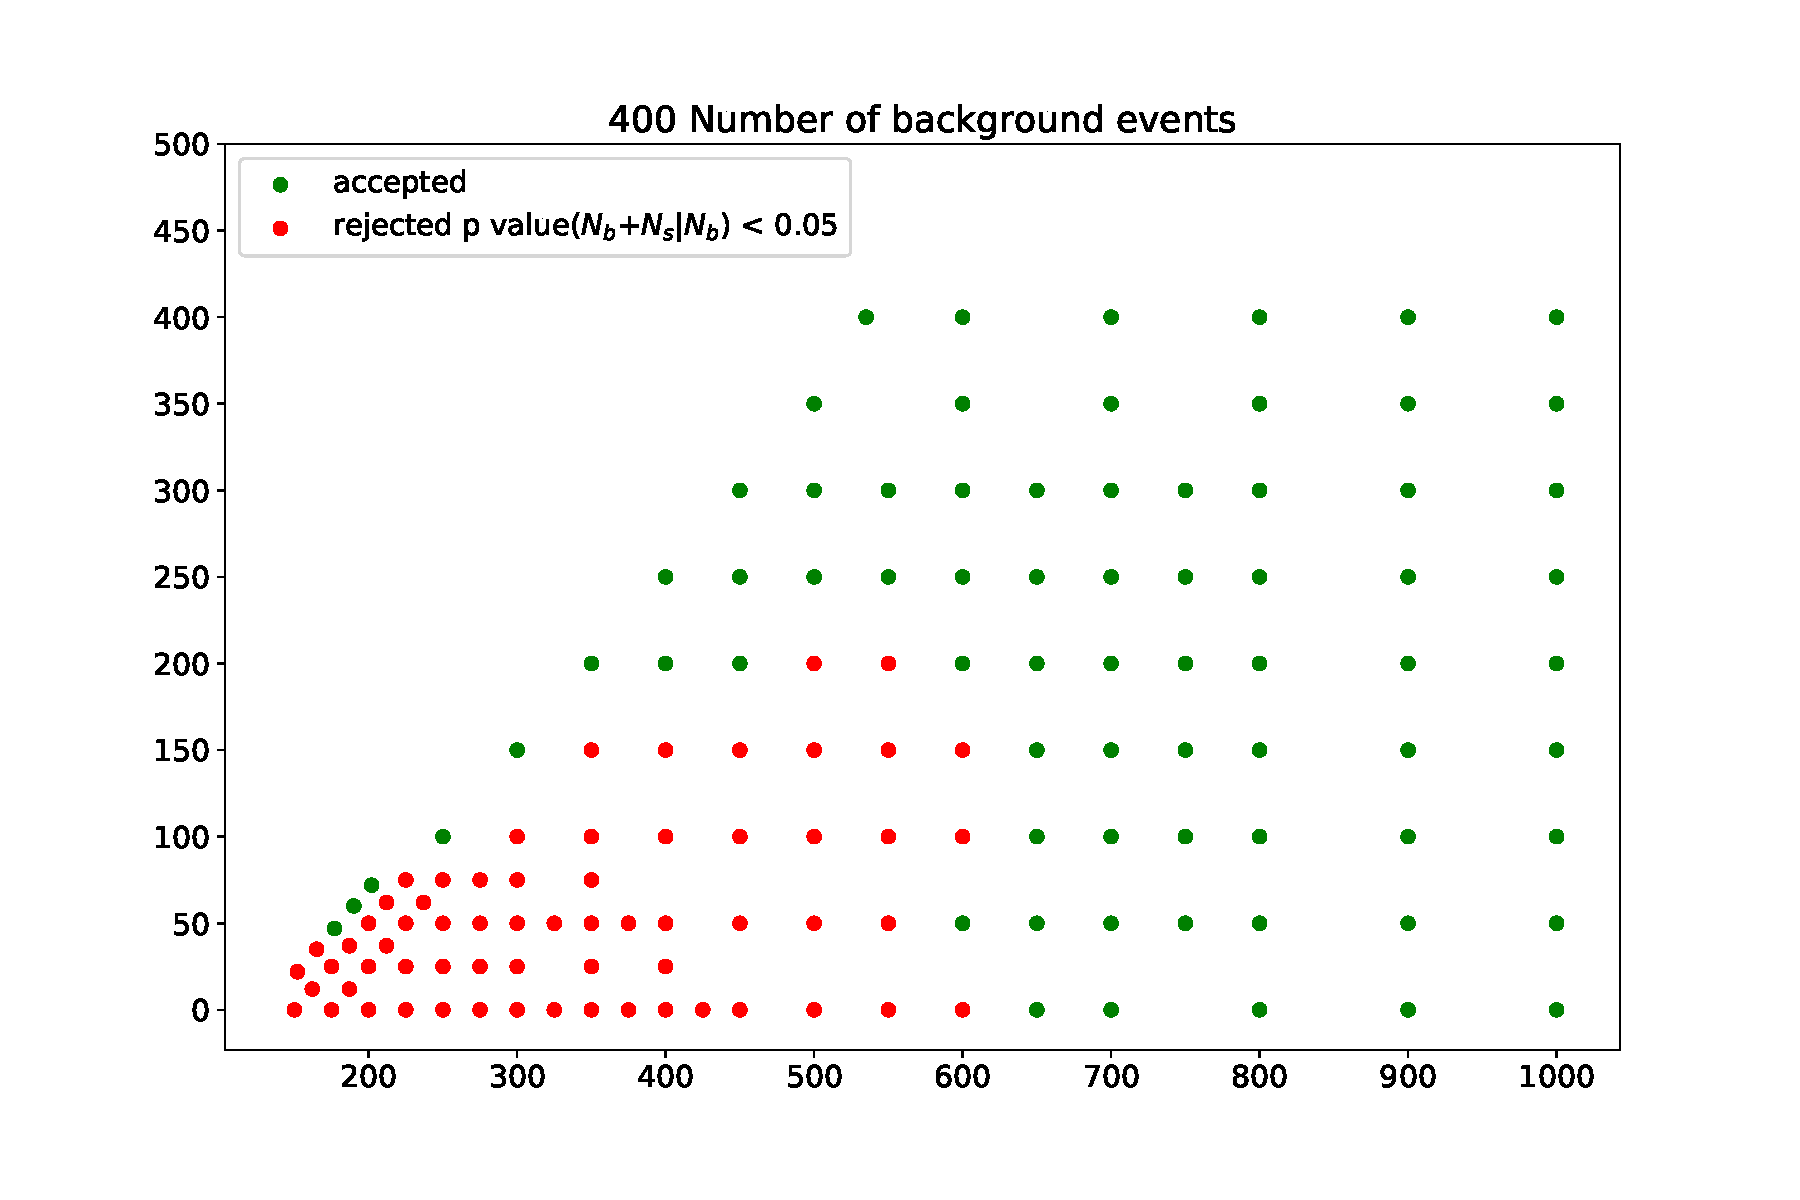
\includegraphics[width=0.71\textwidth]{figs/risultati_simulazione/400.pdf}
	\caption{Risultati degli esperimenti di conteggio per, rispettivamente, 100, 200 e 400 eventi di background selezionati nella parte destra della distribuzione della Loss.}
	\label{test-100-200-400}
\end{figure}

A questo punto vengono individuate tre zone lungo l'asse delle ascisse, rispettivamente per valori $ x \le 300$ , $300 < x \le 600$ e $x > 600$, per poi procedere a verificare in ciascuna zona quale sia il numero ottimale di eventi di background da selezionare nella parte destra della distribuzione in modo da ottimizzare la sensibilità agli eventi di segnale. Da un semplice conteggio dei punti evidenziati in rosso si ottiene che la combinazione ottimale prevede di selezionare 400 eventi di background per la prima zona, 100 per la seconda e 25 per la terza. In figura~\ref{mix} viene riportato l'esito finale dell'esperimento, selezionando per ognuna delle tre zone il valore ottimale di eventi di background da selezionare.

\begin{figure}[h!]
	\centering
	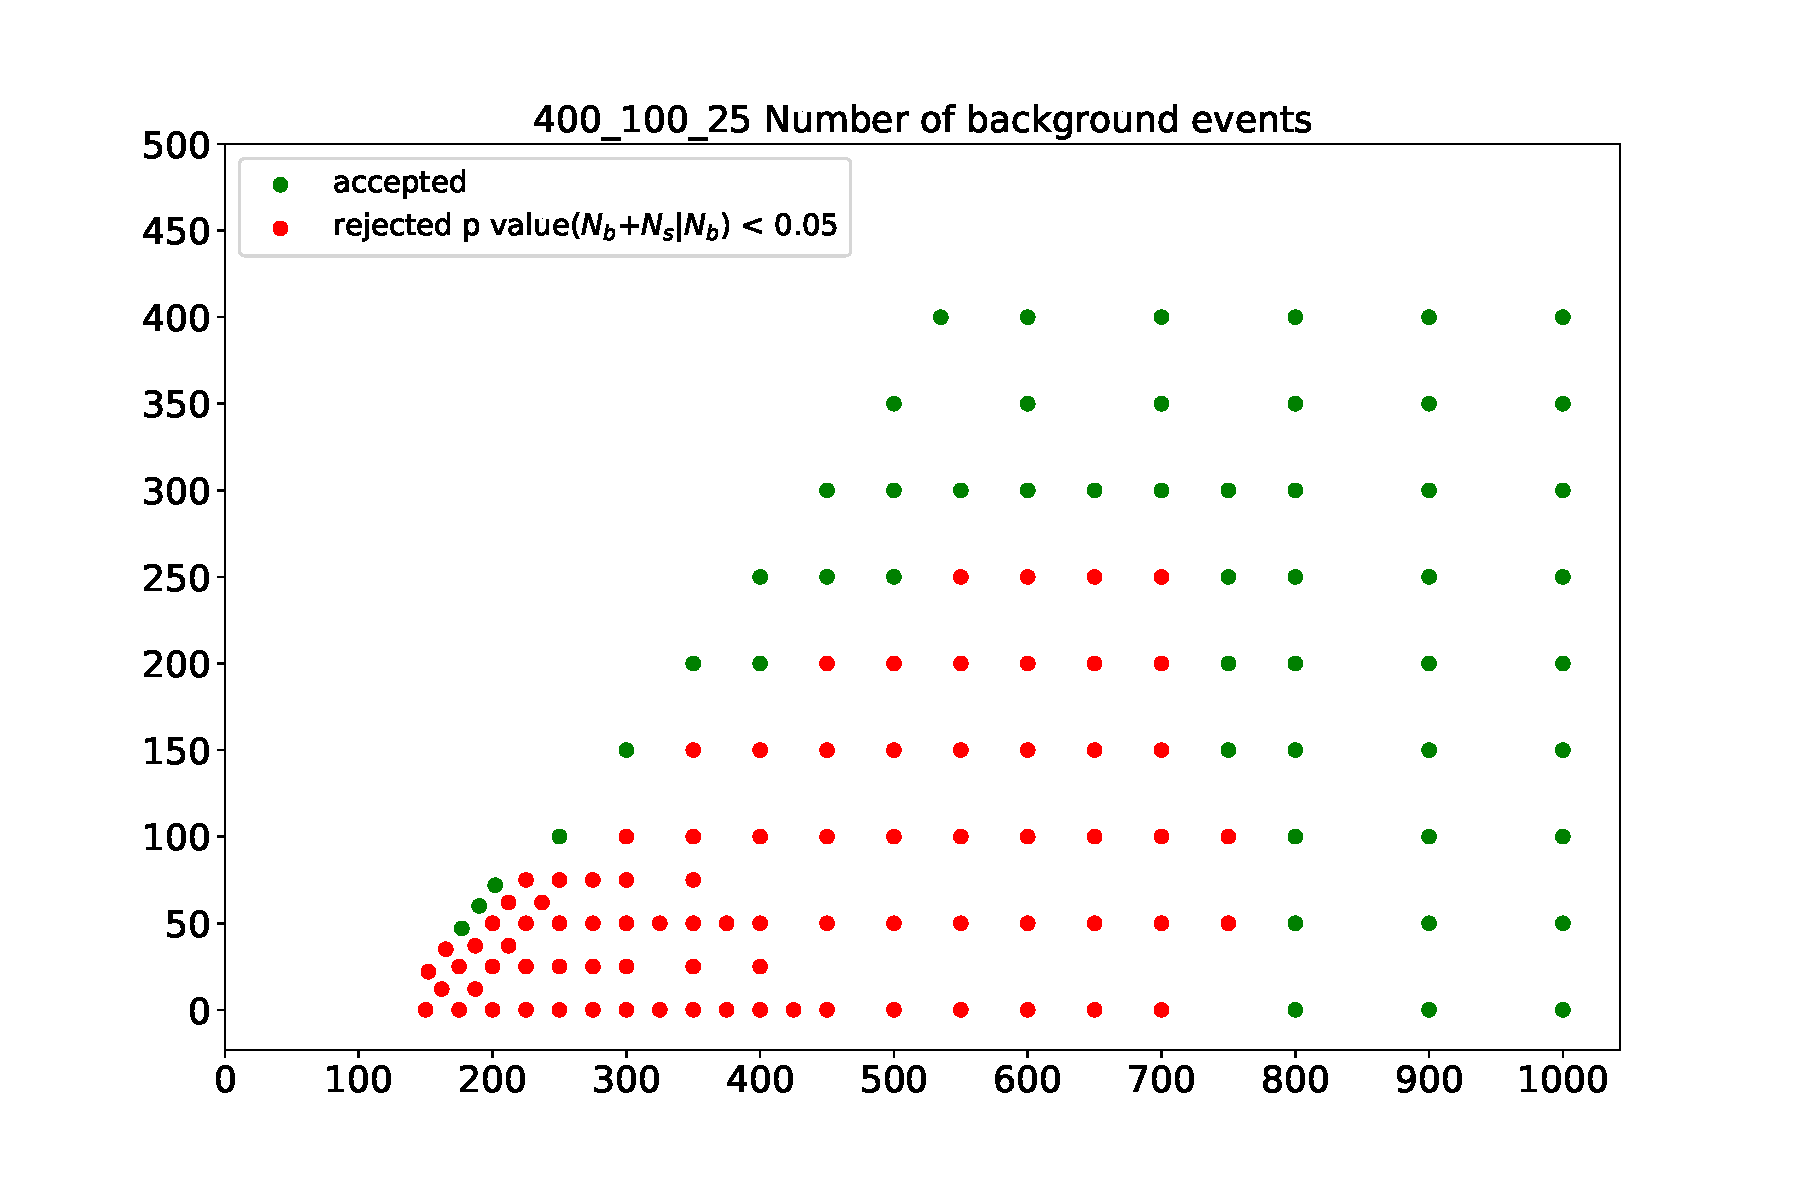
\includegraphics[width=0.90\textwidth]{figs/risultati_simulazione/mix.pdf}
	\caption{Risultato del processo di ottimizzazione nella distinzione fra background e segnale. Sono stati utilizzati i risultati ottimali in ciascuna delle tre zone individuate.}
	\label{mix}
\end{figure}

Quindi il lavoro può considerarsi concluso ma rimangono aperte un paio di domande:
\begin{enumerate}
	\item La ricostruzione della variabile $\textit{mbb}$ non è ottimale; esiste un modo per renderla migliore?
	\item E' possibile che nel processo di classificazione alcune variabili abbiano più importanza (siano più discriminanti) di altre? Se la risposta è affermativa, come si può mettere in evidenza questo fatto?
\end{enumerate} 
A queste domande si cercherà di rispondere nella prossima sezione.\\

\newpage

\subsection{Effetti della variazione degli iperparametri nel processo di apprendimento}
\label{effetti variazione iperparametri}

Come visto nella sezione precedente, sono rimaste aperte un paio di domande alle quali si cercherà di dare una risposta. Per fare ciò bisogna provare a variare gli iperparametri del modello (già incontrati nella sezione~\ref{iperparametri e grid search}); in questo caso gli iperparametri sono i pesi delle otto variabili che vengono impostati all'inizio del processo di apprendimento. Nella sezione precedente si è fatta la scelta più ovvia, ovvero quella di impostare tutti i pesi uguali fra loro e pari ad uno, ma tale configurazione degli iperparametri ha lasciato a desiderare in alcuni punti. \\
In primo luogo è emerso che, nel processo di ricostruzione dei pattern da parte del VAE, il risultato per una delle otto variabili ($\textit{mbb}$) non è stato soddisfacente. Per questo motivo si è provato ad impostare un peso maggiore per questa variabile ed il risultato è riportato in figura~\ref{mbb_ottimizzazione} (nello specifico è stato scelto un peso pari a tre per la variabile $\textit{mbb}$ e ad uno per le altre).

\begin{figure}[h!]
	\centering
	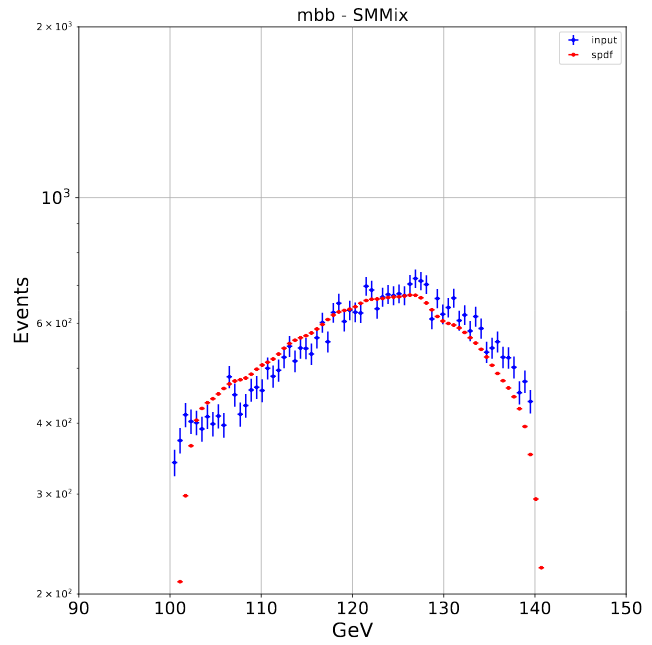
\includegraphics[width=0.65\textwidth]{figs/risultati_simulazione/verifica_mbb.png}
	\caption{Esito del processo di ricostruzione della variabile $\textit{mbb}$ dopo aver impostato un peso pari a tre per tale variabile e mantenendo quelli delle altre variabili pari ad uno. In blu sono riportati i dati originali ed in rosso quelli ricostruiti.}
	\label{mbb_ottimizzazione}
\end{figure}

Risulta evidente che questo piccolo accorgimento in fase di simulazione ha permesso di ottenere un'ottima ricostruzione della variabile $\textit{mbb}$, mantenendo inalterata la qualità delle altre. 

\newpage

Si passa ora a verificare se nel processo di classificazione in segnale e background vi siano alcune variabili più discriminanti di altre; per far emergere ciò bisogna assegnare pesi diversi alle diverse variabili e osservare il conseguente risultato: emerge che ci sono effettivamente tre variabili più discriminanti delle altre, ovvero $\textit{met}$, $\textit{mt}$ e $\textit{mct2}$). Nello specifico sono stati assegnati i pesi rispettivamente pari a 5,10,10 a queste tre variabili ed il risultato finale ottenuto è stato riportato in figura~\ref{mix_ottimizzato}, per poter essere confrontato con il risultato in figura~\ref{mix} dove i pesi erano tutti pari ad uno.

\begin{figure}[h!]
	\centering
	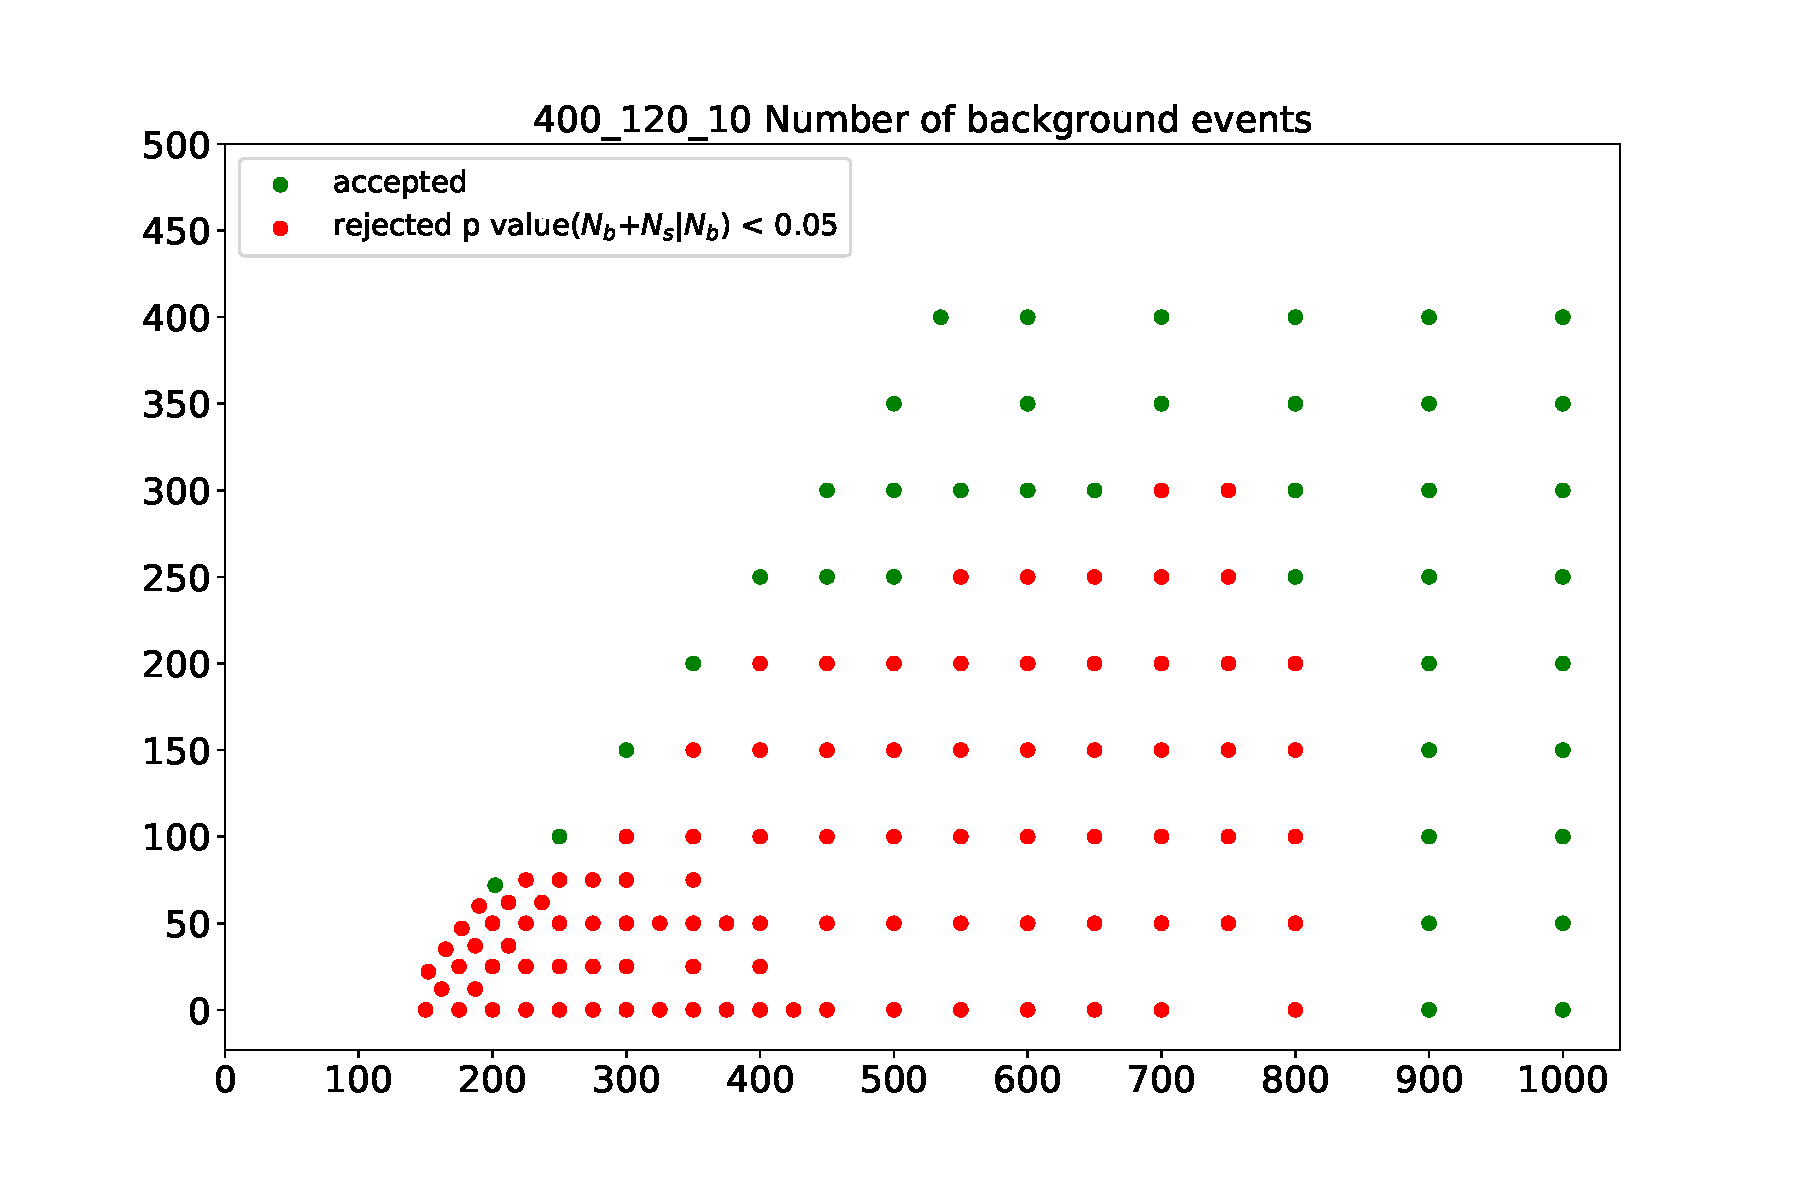
\includegraphics[width=0.90\textwidth]{figs/risultati_simulazione/mix_ottimizzato.pdf}
	\caption{Risultato analogo a quello riportato in figura~\ref{mix}, ma utilizzando pesi differenti per le variabili più discriminanti.}
	\label{mix_ottimizzato}
\end{figure}

Emerge dal confronto fra le due figure che quest'ultima configurazione di iperparametri permette la distinzione del segnale di background per un numero maggiore di possibili combinazioni delle masse delle due particelle. Nel primo caso con pesi tutti pari ad uno il numero totale di combinazioni delle masse delle particelle e quindi di modelli è 82, mentre in questo secondo caso si arriva addirittura a quota 96. \\
Si ottiene quindi una conferma sperimentale di ciò che era già stato introdotto nella sezione~\ref{iperparametri e grid search}, cioè che un modello di apprendimento automatico può essere migliorato andando ad agire sugli iperparametri, ovvero su parametri non soggetti al processo di aggiornamento.

